\documentclass[c]{beamer}  % [t], [c], или [b] --- вертикальное выравнивание на слайдах (верх, центр, низ)

\usetheme{Berlin} % Тема оформления

\usecolortheme{whale} % Цветовая схема
\usepackage[russian]{babel}
\usepackage{hyperref}
\usepackage[usenames,dvipsnames,svgnames,table,rgb]{xcolor}
\hypersetup{				% Гиперссылки
    unicode=true,           % русские буквы в раздела PDF
    colorlinks=true,       	% false: ссылки в рамках; true: цветные ссылки
    linkcolor=violet,          % внутренние ссылки
    citecolor=green,        % на библиографию
    filecolor=magenta,      % на файлы
    urlcolor=pink          % на URL
}

%% Created with wxMaxima 23.05.1

\setlength{\parskip}{\medskipamount}
\setlength{\parindent}{0pt}
\usepackage{iftex}
\ifPDFTeX
  % PDFLaTeX or LaTeX 
  \usepackage[utf8]{inputenc}
  \usepackage[T1]{fontenc}
  \DeclareUnicodeCharacter{00B5}{\ensuremath{\mu}}
\else
  %  XeLaTeX or LuaLaTeX
  \usepackage{fontspec}
\fi
\usepackage{graphicx}
\usepackage{color}
\usepackage{amsmath}
\usepackage{grffile}
\usepackage{ifthen}
\newsavebox{\picturebox}
\newlength{\pictureboxwidth}
\newlength{\pictureboxheight}
\newcommand{\includeimage}[1]{
    \savebox{\picturebox}{\includegraphics{#1}}
    \settoheight{\pictureboxheight}{\usebox{\picturebox}}
    \settowidth{\pictureboxwidth}{\usebox{\picturebox}}
    \ifthenelse{\lengthtest{\pictureboxwidth > .95\linewidth}}
    {
        \includegraphics[width=.75\linewidth,height=.60\textheight,keepaspectratio]{#1}
    }
    {
        \ifthenelse{\lengthtest{\pictureboxheight>.80\textheight}}
        {
            \includegraphics[width=.75\linewidth,height=.60\textheight,keepaspectratio]{#1}
            
        }
        {
            \includegraphics{#1}
        }
    }
}
\newlength{\thislabelwidth}
\DeclareMathOperator{\abs}{abs}

\definecolor{labelcolor}{RGB}{100,0,0}
% \setlength{\topmargin}{-0.5in}
% \setlength{\oddsidemargin}{0 in}
% \textwidth 160mm
% \textheight 220mm

\date{\today}
\institute[ОмГУ]{Омский государственный университет \\ им. Ф.М. Достоевского}
\title{Задания по теории графов}
\author{Рузанова Дарья\\ ММБ-102}
\date{Омск 2024}



\begin{document}

\frame{\titlepage}
\begin{frame}{Задание 1}


% \singlespacing % Reset line spacing to 1 from here on
\setlength{\baselineskip}{8pt}

% \onehalfspacing

Создадим неориентированный граф $G = (V,E)$:

%%%% OUTPUT:
\[\displaystyle 
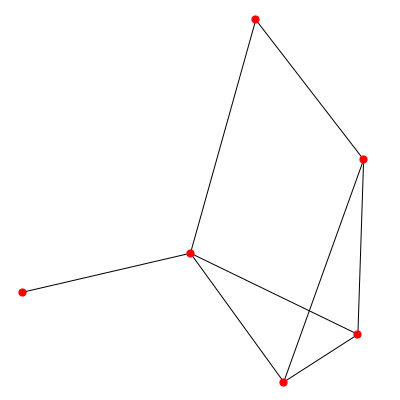
\includegraphics[width=.75\linewidth,height=.60\textheight,keepaspectratio]{graphs_img/graphs_1}\mbox{}
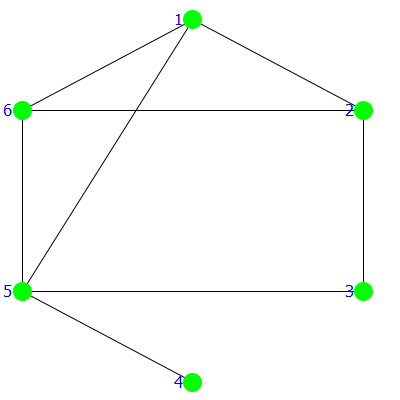
\includegraphics[width=.75\linewidth,height=.60\textheight,keepaspectratio]{graphs_img/graphs_2}\mbox{}\]
\end{frame}
\begin{frame}
\frametitle{Задание 1}
Дополнение $\overline{G}$ графа $G$:\\


\[\displaystyle 
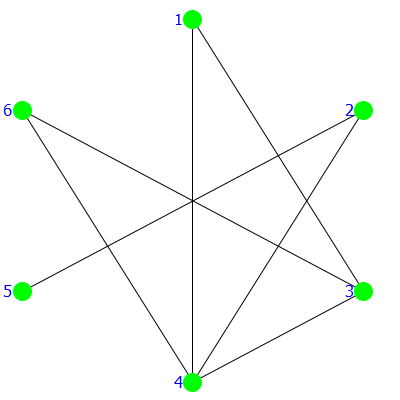
\includegraphics[width=.75\linewidth,height=.60\textheight,keepaspectratio]{graphs_img/graphs_3}\mbox{}\]
\end{frame}


\begin{frame}
\frametitle{Задание 1}
Матрица смежности графа $G$:\\


%%%%%%%%
%% INPUT:
\[\displaystyle
\begin{pmatrix}0 & 1 & 0 & 0 & 1 & 1\\
1 & 0 & 1 & 0 & 0 & 1\\
0 & 1 & 0 & 0 & 1 & 0\\
0 & 0 & 0 & 0 & 1 & 0\\
1 & 0 & 1 & 1 & 0 & 1\\
1 & 1 & 0 & 0 & 1 & 0\end{pmatrix}\mbox{}
\]
%%%%%%%%%%%%%%%%
\end{frame}
\begin{frame}
\frametitle{Задание 1}
Матрица смежности графа $\overline{G}$:\\

\[\displaystyle
\begin{pmatrix}0 & 0 & 1 & 1 & 0 & 0\\
0 & 0 & 0 & 0 & 1 & 0\\
1 & 0 & 0 & 1 & 1 & 1\\
1 & 0 & 1 & 0 & 0 & 1\\
0 & 1 & 1 & 0 & 0 & 0\\
0 & 0 & 1 & 1 & 0 & 0\end{pmatrix}\mbox{}
\]
%%%%%%%%%%%%%%%%
\end{frame}

\begin{frame}{Задание 2}

Создадим граф $G_1$ по его матрице смежности \\
$$
\left[\begin{array}{cccccc}
    0 & 1 & 1 & 0 & 0 & 0\\
    1 & 0 & 1 & 0 & 1 & 1\\
    1 & 1 & 0 & 0 & 0 & 0\\
    0 & 0 & 0 & 0 & 1 & 0\\
    0 & 1 & 0 & 1 & 0 & 1\\
    0 & 1 & 0 & 0 & 1 & 0
\end{array}\right]$$
\end{frame}

\begin{frame}
\frametitle{Задание 2}
Граф $G_1$:\\


\[\displaystyle  
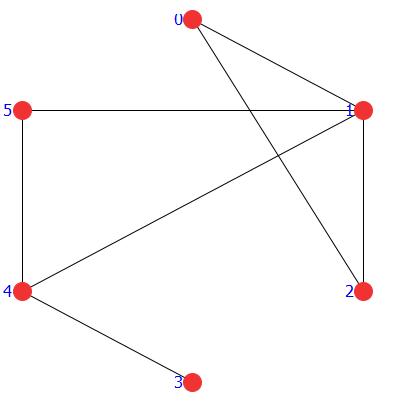
\includegraphics[width=.75\linewidth,height=.60\textheight,keepaspectratio]{graphs_img/graphs_4}\mbox{}\]
\end{frame}

\begin{frame}{Задание 3}

Создадим орграф $G_2$ по заданным спискам вершин и ребер.\\

\[\displaystyle
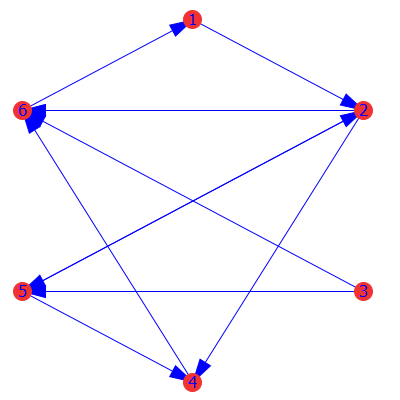
\includegraphics[width=.75\linewidth,height=.60\textheight,keepaspectratio]{graphs_img/graphs_5}\mbox{}\]
\end{frame}

%%%%%%%%%%%%%%%%
\begin{frame}
\frametitle{Задание 3}
Матрица смежности $G_2$:\\


\[\displaystyle
\begin{pmatrix}0 & 0 & 0 & 0 & 0 & 1\\
1 & 0 & 0 & 0 & 1 & 0\\
0 & 0 & 0 & 0 & 0 & 0\\
0 & 1 & 0 & 0 & 1 & 0\\
0 & 1 & 1 & 0 & 0 & 0\\
0 & 1 & 1 & 1 & 0 & 0\end{pmatrix}\mbox{}
\]
\end{frame}
%%%%%%%%%%%%%%%%

\begin{frame}{Задание 4}

Пустой 5-вершинный граф $O_9$:
\\
\[
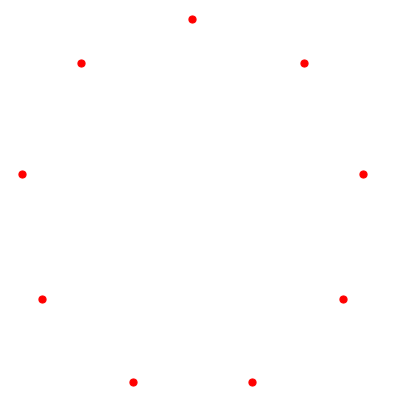
\includegraphics[width=.75\linewidth,height=.60\textheight,keepaspectratio]{graphs_img/graphs_6}\mbox{}\]
\end{frame}

\begin{frame}
\frametitle{Задание 4}
Полный 6-вершинный граф $K_{6}$:\\

\[
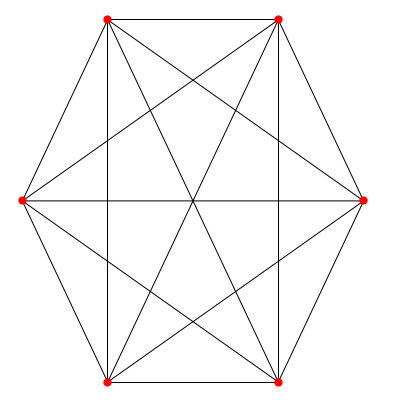
\includegraphics[width=.75\linewidth,height=.60\textheight,keepaspectratio]{graphs_img/graphs_7}\mbox{}\]
\end{frame}

%%%%%%%%%%%%%%%%

\begin{frame}
\frametitle{Задание 4}
Полный двудольный граф $K_{3,5}$:\\

\[
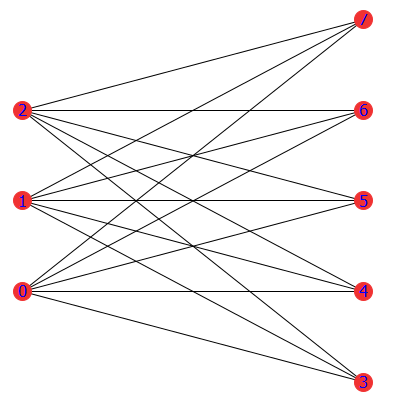
\includegraphics[width=.75\linewidth,height=.60\textheight,keepaspectratio]{graphs_img/graphs_8}\mbox{}\]
\end{frame}

\begin{frame}
\frametitle{Задание 4}
Создадим простую цепь $P_{6}$ и построим её изображение:\\

\[
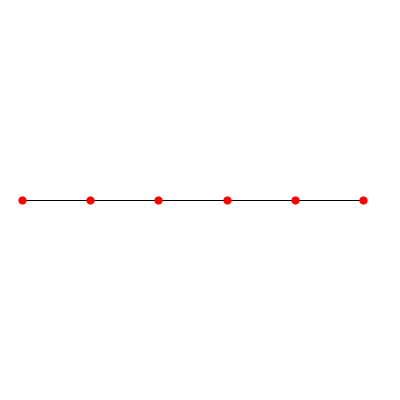
\includegraphics[width=.75\linewidth,height=.60\textheight,keepaspectratio]{graphs_img/graphs_9}\mbox{}\]
\end{frame}
\begin{frame}
\frametitle{Задание 4}
Простой 5-вершинный цикл $C_{9}$:\\

\[
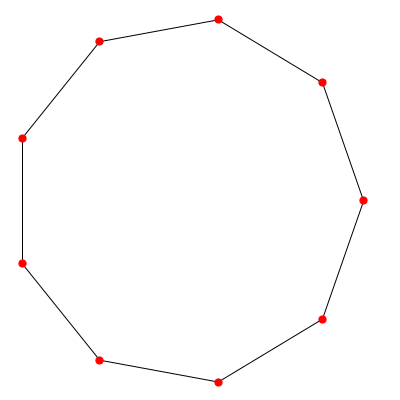
\includegraphics[width=.75\linewidth,height=.60\textheight,keepaspectratio]{graphs_img/graphs_10}\mbox{}\]
\end{frame}

\begin{frame}
\frametitle{Задание 4}
Граф куба $Q_{4}$:\\


\[
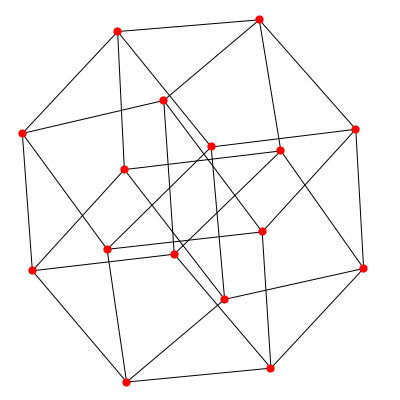
\includegraphics[width=.75\linewidth,height=.60\textheight,keepaspectratio]{graphs_img/graphs_11}\mbox{}\]
\end{frame}

%%%%%%%%%%%%%%%%
\begin{frame}
\frametitle{Задание 4}
Граф колеса $W_9$ :\\

\[
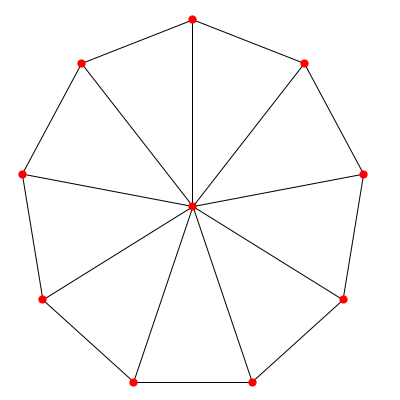
\includegraphics[width=.75\linewidth,height=.60\textheight,keepaspectratio]{graphs_img/graphs_12}\mbox{}\]
\end{frame}
%%%%%%%%%%%%%%%%
\begin{frame}
\frametitle{Задание 4}
Граф Петерсена:\\

\[
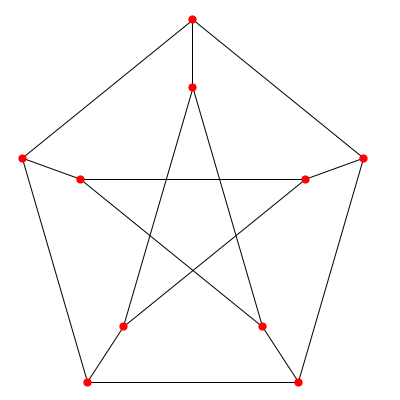
\includegraphics[width=.75\linewidth,height=.60\textheight,keepaspectratio]{graphs_img/graphs_13}\mbox{}\]
\end{frame}

%%%%%%%%%%%%%%%%

\begin{frame}{Задание 5}

Случайный граф с 6 вершинами, каждое ребро которого присутствует с вероятностью 0,7:\\
\[
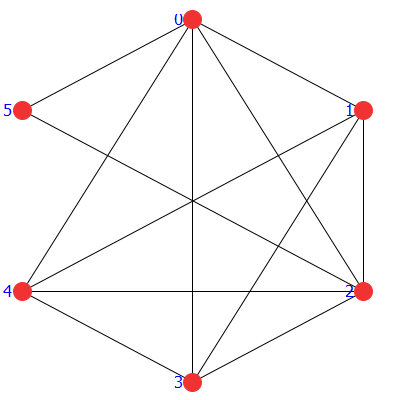
\includegraphics[width=.75\linewidth,height=.60\textheight,keepaspectratio]{graphs_img/graphs_14}\mbox{}\]
\end{frame}
%%%%%%%%%%%%%%%%
\begin{frame}
\frametitle{Задание 5}
Случайный орграф с 8 вершинами, каждое ребро которого присутствует с вероятностью 0,3:\\

\[
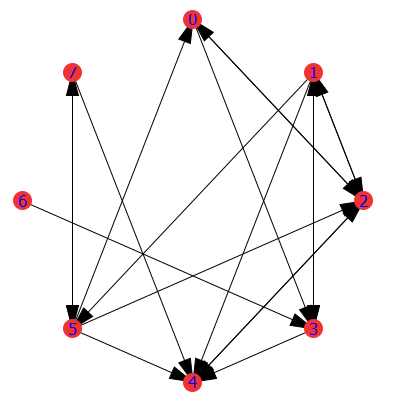
\includegraphics[width=.75\linewidth,height=.60\textheight,keepaspectratio]{graphs_img/graphs_15}\mbox{}\]
\end{frame}
%%%%%%%%%%%%%%%%

\begin{frame}{Задание 6}


Случайный двудольный граф с числом вершин $5+7$, каждое ребро которого присутствует с вероятностью 0,6:\\
\[
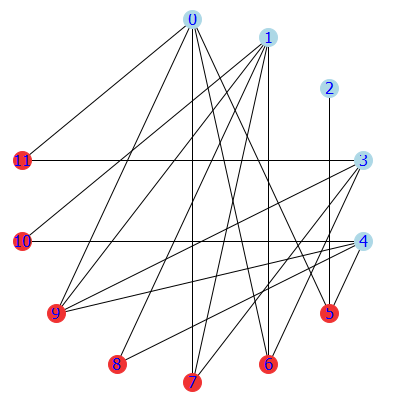
\includegraphics[width=.75\linewidth,height=.60\textheight,keepaspectratio]{graphs_img/graphs_16}\mbox{}\]
\end{frame}
%%%%%%%%%%%%%%%%

\begin{frame}{Задание 7}


Случайный граф F с 20 вершинами и 100 ребрами:\\
\noindent


\[
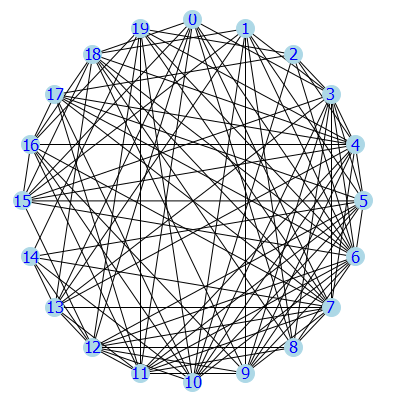
\includegraphics[width=.75\linewidth,height=.60\textheight,keepaspectratio]{graphs_img/graphs_17}\mbox{}\]
\end{frame}

\begin{frame}
\frametitle{Задание 7}
Граф $F$ является связным,\\
но не является деревом, двудольным и планарным.\\ \\

Гамильтонов цикл этого графа: 
\[\displaystyle 
\left[ 0\operatorname{,}1\operatorname{,}2\operatorname{,}3\operatorname{,}4\operatorname{,}5\operatorname{,}6\operatorname{,}7\operatorname{,}8\operatorname{,}9\operatorname{,}10\operatorname{,}11\operatorname{,}12\operatorname{,}13\operatorname{,}14\operatorname{,}15\operatorname{,}16\operatorname{,}17\operatorname{,}18\operatorname{,}19\right] \mbox{}
\]

\end{frame}


\begin{frame}
\frametitle{Задание 7}
Cписок вершин:
%%%% OUTPUT:
\[\displaystyle
\left[ 0\operatorname{,}1\operatorname{,}2\operatorname{,}3\operatorname{,}4\operatorname{,}5\operatorname{,}6\operatorname{,}7\operatorname{,}8\operatorname{,}9\operatorname{,}10\operatorname{,}11\operatorname{,}12\operatorname{,}13\operatorname{,}14\operatorname{,}15\operatorname{,}16\operatorname{,}17\operatorname{,}18\operatorname{,}19\right] \mbox{}
\]
%%%%%%%%%%%%%%%%


%%%%%%%%
%% INPUT:
Cписок ребер:

%%%% OUTPUT:
\[\displaystyle 
\operatorname{[}\left[ 0\operatorname{,}3\right] \operatorname{,}\left[ 0\operatorname{,}6\right] \operatorname{,}\left[ 0\operatorname{,}7\right] \operatorname{,}\left[ 0\operatorname{,}8\right] \operatorname{,}\left[ 0\operatorname{,}11\right] \operatorname{,}\left[ 0\operatorname{,}12\right] \operatorname{,}\left[ 0\operatorname{,}13\right] \operatorname{,}\left[ 0\operatorname{,}15\right] \operatorname{,}\left[ 0\operatorname{,}18\right] \operatorname{,
} ...]\]

Список степеней вершин:

%%%% OUTPUT:
\[\displaystyle  
\left[ 6\operatorname{,}6\operatorname{,}8\operatorname{,}8\operatorname{,}9\operatorname{,}9\operatorname{,}9\operatorname{,}9\operatorname{,}9\operatorname{,}9\operatorname{,}10\operatorname{,}10\operatorname{,}11\operatorname{,}11\operatorname{,}12\operatorname{,}12\operatorname{,}12\operatorname{,}13\operatorname{,}13\operatorname{,}14\right] \mbox{}
\]
%%%%%%%%%%%%%%%%
\end{frame}
\begin{frame}
\frametitle{Задание 7}

Средняя степень вершин графа $F$:      11\\
Минимальная:      6, у вершины номер 2\\
Максимальная:      14, у вершины номер 6\\
Степень вершины 10:     11\\
Список вершин, смежных с вершиной 10:

\[\displaystyle 
\left[ 1\operatorname{,}2\operatorname{,}3\operatorname{,}4\operatorname{,}5\operatorname{,}6\operatorname{,}12\operatorname{,}14\operatorname{,}16\operatorname{,}17\operatorname{,}19\right] \mbox{}
\]
\end{frame}
%%%%%%%%%%%%%%%%
\begin{frame}
\frametitle{Задание 7}
Диаметр графа F: 2\\
Периферия:
\[\displaystyle \tag{\% o55} 
\left[ 19\operatorname{,}18\operatorname{,}17\operatorname{,}16\operatorname{,}15\operatorname{,}14\operatorname{,}13\operatorname{,}12\operatorname{,}11\operatorname{,}10\operatorname{,}9\operatorname{,}8\operatorname{,}7\operatorname{,}6\operatorname{,}5\operatorname{,}4\operatorname{,}3\operatorname{,}2\operatorname{,}1\operatorname{,}0\right] \mbox{}\]
Радиус графа: 2\\
Центр графа:
\[
\left[ 19\operatorname{,}18\operatorname{,}17\operatorname{,}16\operatorname{,}15\operatorname{,}14\operatorname{,}13\operatorname{,}12\operatorname{,}11\operatorname{,}10\operatorname{,}9\operatorname{,}8\operatorname{,}7\operatorname{,}6\operatorname{,}5\operatorname{,}4\operatorname{,}3\operatorname{,}2\operatorname{,}1\operatorname{,}0\right] \mbox{}\]
Эксцентриситет вершины 10: 2\\

\end{frame}
%%%%%%%%%%%%%%%%
\begin{frame}{Задание 8}

Случайный орграф H c 20 вершинами, каждая дуга которого присутствует с вероятностью 0,6:\\


\[
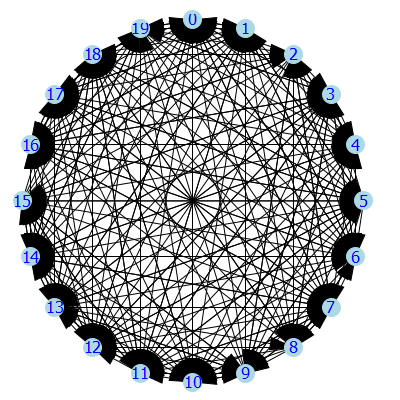
\includegraphics[width=.75\linewidth,height=.60\textheight,keepaspectratio]{graphs_img/graphs_18}\mbox{}\]
\end{frame}

\begin{frame}
\frametitle{Задание 8}
$H$ является \textbf{сильно связным}.\\
Степень захода вершины 10: 13 \\
Степень исхода вершины 10: 7

\end{frame}

\begin{frame}{Заключение}

\textbf{Цель исследования: } познакомиться с специализированным пакетом $graphs$, создать различные графы, изобразить их и исследовать их свойства. \\

\textbf{Использованные средства: }программа wxMaxima.\\


Были построены их изображения с опциями по умолчанию и заданными. Были найдены матрицы смежности некоторых графов.
\end{frame}
\begin{frame}
\frametitle{Заключение}
\textbf{Результат: } 
\begin{enumerate}
    \item Были созданы различные графы и орграфы разными способами;
    \item Были построены их изображения;
    \item Найдены матрицы смежности некоторых графов;
    \item Изучены некоторые свойства графов $F$ и $H$.
\end{enumerate}
\end{frame}
\end{document}
